\documentclass[12pt]{article}
\usepackage[utf8]{inputenc}
\usepackage[T1]{fontenc}

\usepackage{mathptmx}

\title{Analysing Orphaned Triples in a Large-Scale Graph Database}
\author{Gary Gurlaskie}
\date{15 April 2020}

\usepackage[]{geometry}
\usepackage{natbib}
\usepackage{graphicx}
\usepackage{url}
\usepackage{xcolor}
\usepackage{listings}
\usepackage[parfill]{parskip}
\lstset{basicstyle=\footnotesize\ttfamily,breaklines=true}

\begin{document}

\begin{titlepage}
 \centering
 \vspace*{1in}
 \begin{Large}\bfseries
  Analyzing Orphaned Triples in a Large-Scale Graph Database\par
 \end{Large}

  CIS4914 -- Final Report\par
  Spring 2020\par

  \vspace*{0.2in}
  
  Gary Gurlaskie (\url{g.gurlask@ufl.edu})\par
  Individual Project\par
  16 April 2020\par
\end{titlepage}

\section*{Abstract}
This project emphasized data analysis and visualization, and was focused on UF VIVO, an 7.1 GB RDF graph database that documents UF research efforts. The goal was to identify data in VIVO that had become "orphaned" (disconnected) from the graph.

The analysis was performed ad hoc using Python. Analysis performed included examining zero- or low-degree nodes, orphaned connected components, and performing constraint validation against the published ontology.

The work yielded over 10,000 orphaned triples. However, the quality of the data was high overall; 94\% of the graph was connected in a robust way.

\section*{Introduction}

\begin{lstlisting}
a := 1;
\end{lstlisting}

\begin{figure}[h!]
\centering
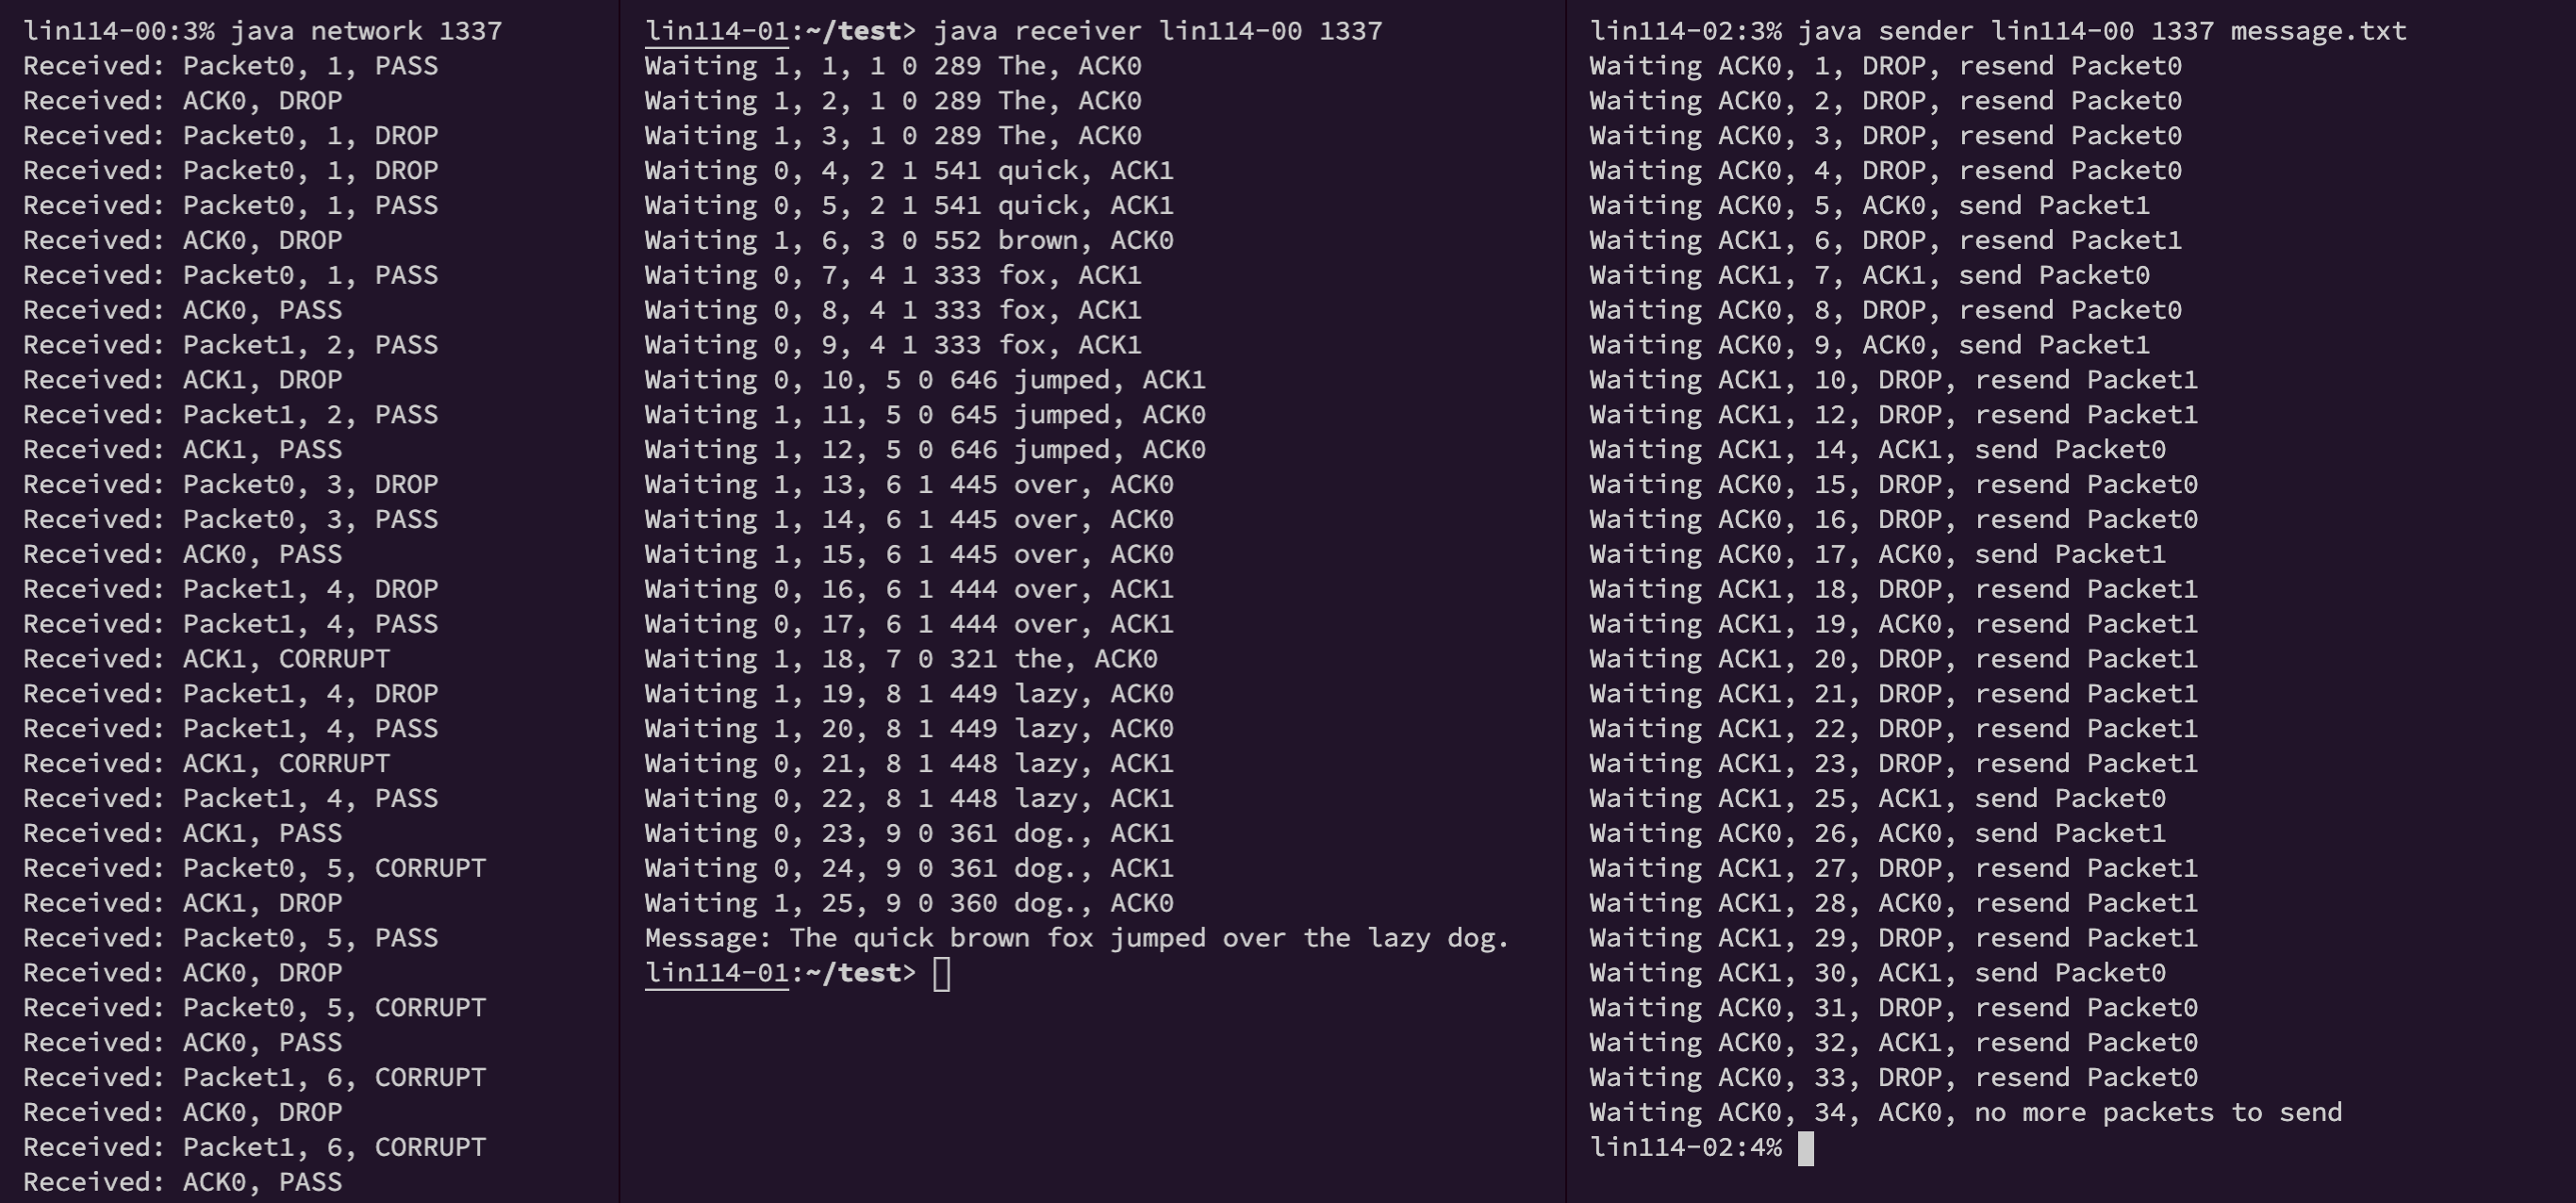
\includegraphics[width=\textwidth]{output.png}
\caption{An example execution.}
\label{fig:output}
\end{figure}

\section*{Acknowledgments}
The author thanks Christopher Barnes for advising the project, and the UF CTS-IT for providing access to the VIVO data. The author also thanks Taeber Rapczak for his excellent help and guidance.

\section*{Biography}
Gary Gurlaskie is an undergraduate student studying Mathematics and Computer Science at the University of Florida. He worked at Ultimate Software (data platform engineering) and Intel (software engineering). He plans to graduate in May 2020, and upon graduation will move to Portland to work at Intel full-time. He has always wanted to have a cat, so he will obtain one when he moves to Oregon.

\end{document}

